\documentclass[a4paper]{article}

\usepackage[english]{babel}
\usepackage[utf8x]{inputenc}
\usepackage{amsmath}
\usepackage{graphicx}
\usepackage{multicol}
\usepackage{tikz}
\usetikzlibrary{matrix,chains,positioning,decorations.pathreplacing,arrows}
\usepackage[colorinlistoftodos]{todonotes}
\usepackage[pagebackref=true,breaklinks=true,letterpaper=true,colorlinks,bookmarks=false,linktoc=all]{hyperref}

\usepackage{titlesec}
\hypersetup{
    colorlinks,
    citecolor=black,
    filecolor=black,
    linkcolor=black,
    urlcolor=black
}

\title{Back propagation reference}
%\author{Aaron Wetzler, Dor Verbin}

\begin{document}
\maketitle

\begin{abstract}
This document serves as a reference for students, engineers and researchers who occasionally need to work through the analytic computation of gradients and back-propagation update calculations. The document is an ongoing effort and there may be errors. Please feel free to send pull requests with new layers or corrections.
\end{abstract}

\tableofcontents
\newpage
\section{Intro}
\begin{figure}\label{fig:general}
\centering
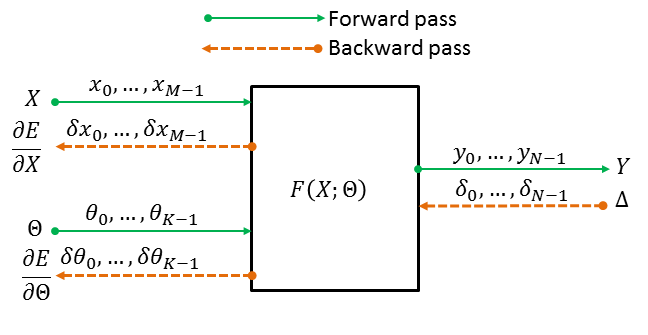
\includegraphics[width=0.75\textwidth]{ForwardBackward.png}
\caption{This image illustrates a general view of a network layer that is useful to understand back propagation. The layer takes inputs $X$, parameters $\Theta$ and produces an output $Y$. Computing the output is performed during the forward pass. Updating the parameters and passing the error signal $\Delta$ back from the next layer is performed during the backward pass.}
\end{figure}
We will consider here the most general function description of a neural network layer where the network takes in a multi-dimensional input $X$ and a set of tunable parameters $\Theta$. It produces a multi-dimensioanl output $Y$. When $X,Y,\Theta$ are scalars we will refer to them as $x,y,\theta$. Instead of $\Theta$ and $\theta$ we may also use $W,w,B,b$ if the context is related to convolution. Figure \ref{fig:general} illustrates this setup. We will try to preserve this notation throughout the document to aid in understanding and implementation. Each Section is intended to be independent of the others although there may be cross referencing.

%+++++++++++++++++++++++++++++++++++++++++++++++++++++++++++++++
\newpage
\section{Neuron activation functions}
Neuron activation functions take a single input and produce a single output. There are two groups of such functions: those with tunable parameters and those without. However in the general case we can write down the following function
\begin{equation}
y = f(x,\theta),
\end{equation}
where $x$ is a scalar input, $y$ is a scalar output and $\theta$ is a vector of tunable parameters. The backprop equations here are 
\begin{align} \label{eq:elementwise}
\frac{\mathrm{d} E }{\mathrm{d} x} = & \delta \frac{\mathrm{d} f(x,\theta)}{\mathrm{d} x}\\
\frac{\partial E }{\partial \theta_i} = & \delta \frac{\partial f(x,\theta)}{\partial \theta_i}.
\end{align}

%---------------------------------------------------------------
\subsection{ReLU}
The {\bf Re}ctified {\bf L}inear {\bf U}nit function is given by
\begin{equation}
f(x)=\left\{\begin{matrix}
 & 0 & x< 0\\ 
 & x & x \geq 0
\end{matrix}\right.
\end{equation}
Finding its derivative is straightforward. We simply find the derivative for each section in its domain. We can directly compute the backprop gradient
\begin{align}
\frac{\mathrm{d} E }{\mathrm{d} x}= &\delta \frac{\mathrm{d} f }{\mathrm{d} x} \\
= & \delta \left\{\begin{matrix}
 & 0 & x< 0\\ 
 & 1 & x \geq 0
\end{matrix}\right. \\
= & \left [ \delta \right ]_{x \geq 0}
\end{align}
In other words ReLU acts like an on/off switch for error signals. If the input $x$ was greater than or equal to zero then the error signal $\delta$ will be passed back to the next layer down. If not then no error signal will be funneled through and anything behind this neuron will not be updated. 
%---------------------------------------------------------------
\subsection{Leaky ReLU}
%---------------------------------------------------------------
\subsection{TanH}
For the hyperbolic tangent function (or TanH), 
\begin{equation}
f(x)=\tanh(x)=\frac{e^{x}-e^{-x}}{e^{x}+e^{-x}}
\end{equation}
Finding its derivative can be done using the quotient rule,
\begin{align}
\frac{\mathrm{d}f}{\mathrm{d}x}
= & \frac{\mathrm{d}}{\mathrm{d}x}\frac{e^{x}-e^{-x}}{e^{x}+e^{-x}}\\
= & \frac{(e^{x}+e^{-x})(e^{x}+e^{-x})-(e^{x}-e^{-x})(e^{x}-e^{-x})}{(e^{x}+e^{-x})^2}\\
= & \frac{(e^{x}+e^{-x})^{2}-(e^{x}-e^{-x})^{2}}{(e^{x}+e^{-x})^2}\\
= & 1 - \left ( \frac{e^{x}-e^{-x}}{e^{x}+e^{-x}} \right )^{2}\\
= & 1 - \left( \tanh(x) \right)^{2}.
\end{align}
Plugging the derivative into equation \ref{eq:elementwise}, we get
\begin{align}
\frac{\mathrm{d} E }{\mathrm{d} x}= &\delta \frac{\mathrm{d} f }{\mathrm{d} x} \\
= & \delta \left ( 1-y^{2} \right ).
\end{align}

%---------------------------------------------------------------
\subsection{Sigmoid}
The Sigmoid function is defined as
\begin{equation}
\sigma (x)= \frac{1}{1+e^{-x}}.
\end{equation}
Its derivative is simply
\begin{align}
\frac{\mathrm{d} \sigma }{\mathrm{d} x}&= - \frac{-e^{-x}}{\left( 1+e^{-x} \right)^{2}} \\
&= \frac{1}{1+e^{-x}}\frac{e^{-x}}{1+e^{-x}} \\
&= \frac{1}{1+e^{-x}}\left(1-\frac{1}{1+e^{-x}}\right)\\
&= \sigma(x)\left(1-\sigma(x)\right).
\end{align}
Plugging the derivative into equation \ref{eq:elementwise}, we get
\begin{align}
\frac{\mathrm{d} E }{\mathrm{d} x}= &\delta \frac{\mathrm{d} \sigma }{\mathrm{d} x} \\
= & \delta y\left ( 1-y \right ).
\end{align}

%---------------------------------------------------------------
\subsection{Absolute value}
%---------------------------------------------------------------
\subsection{Power}


%+++++++++++++++++++++++++++++++++++++++++++++++++++++++++++++++
\newpage
\section{Windowed functions}
The family of functions which considers a window of a spatial input includes among others pooling and convolutional layers. There are often many ways to perform back propagation across these layers and usually depends on the desired performance considerations when implemented in a computer.  To index into our input $X$ which will typically be $C \times H \times W$, we will use the following: $i \in 0 \cdots H-1$ traverses the rows (y direction in image), $j \in 0 \cdots W-1$ traverses the columns (x direction in image) and $c \in 0 \cdots C-1$ traverses the channels (colors or filters direction often called depth).

%---------------------------------------------------------------
\subsection{Max pooling}
Max pooling takes in a 
\begin{equation}
f(X)=\max\limits_{i \in 0 \cdots n} x_i
\end{equation}
%---------------------------------------------------------------
\subsection{Max unpooling}
%---------------------------------------------------------------
\subsection{Average pooling}
%---------------------------------------------------------------
\subsection{Average unpooling}
%---------------------------------------------------------------
\subsection{Mean Variance Normalization (Instance norm)}
%---------------------------------------------------------------
\subsection{Convolution}
%---------------------------------------------------------------
\subsection{Deconvolution(tranposed convolution)}

%+++++++++++++++++++++++++++++++++++++++++++++++++++++++++++++++
\newpage
\section{Restructuring functions}
There are numerous cases where the structure of the input data need to be adjusted such as flattening, cropping, padding, resizing and more. In these cases the challenge is to figure out how to perform back prop on the data which has been moved around, cut off or added. 
%---------------------------------------------------------------
\subsection{Padding}
%---------------------------------------------------------------
\subsection{Cropping}

%+++++++++++++++++++++++++++++++++++++++++++++++++++++++++++++++
\newpage
\section{Loss functions}
%---------------------------------------------------------------
\subsection{Euclidean}
The Euclidean loss is defined by the average of the square of the residuals and is written as
\begin{equation}
E(X,Y) = \frac{1}{CHW}\sum_{i,j,k}^{C,H,W} \frac{1}{2}\left (  X_{ijk} - Y_{ijk}\right )^2
\end{equation}
where here we arbitrarily assume an input $X$ with three dimensions and an output $Y$ with the same structure. 
The loss function gradient which then typically becomes the first set of error signals $\Delta$ can be written as
\begin{align}
\delta_{cmn} 
= &\frac{\partial E}{\partial X_{cmn}} \\
= &\frac{1}{CHW}\sum_{i,j,k}^{C,H,W} \left (  X_{ijk} - Y_{ijk}\right ) \frac{X_{ijk}}{\partial X_{cmn}} \\
= &\frac{1}{CHW}\left (  X_{cmn} - Y_{cmn}\right )
\end{align}
or in matrix form
\begin{equation}
\Delta = \frac{1}{CHW}\left (  X - Y\right )
\end{equation}
%---------------------------------------------------------------
\subsection{Cross entropy}
%---------------------------------------------------------------
\subsection{Discrete total variation}

The discrete total variation can be written as 
\begin{equation}
TV(X)= \sum_{i,j} \left ( \left ( X_{ij+1}-X_{ij}\right )^2 + \left ( X_{i+1j}-X_{ij}\right )^2 \right )^{1/2}= \sum_{i,j} \left | \nabla_{ij} X \right |_2 ,
\end{equation}
where $i \in (0\dots H-1)$ and $j \in (0\dots W-1)$. $X$ is used to represent the image and has dimensions $H \times W$. For the sake of simplicity we will assume a single channel because the result shown here will simply be redone for all channels and all examples in a batch. In this case the {\it total variation} is a loss and therefore our backprop update only requires that we compute the gradient of $TV$ with respect to the image. Also note that for convenience of notation we use $\left | \nabla_{ij} X \right |_2$ to indicate the magnitude of the forward discrete derivative at $(ij)$.

\begin{align}
\begin{split}
\frac{\partial{E}}{\partial{X_{mn}}} = & \frac{\partial{TV(X)}}{\partial{X_{mn}}} \\
 = & \sum_{i,j} \frac{\partial \left | \nabla_{ij} X \right |_2}{\partial X_{mn}}\\
 = & \sum_{i,j} \frac{1}{2}\frac{1}{ \left | \nabla_{ij} X \right |_2}\left [ 2(X_{ij+1}-X{ij})(\frac{\partial X_{ij+1}}{\partial X_{mn}} - \frac{\partial X_{ij}}{\partial X_{mn}}) + 2(X_{i+1j}-X{ij})(\frac{\partial X_{i+1j}}{\partial X_{mn}} - \frac{\partial X_{ij}}{\partial X_{mn}}) \right ] \\
  = & 
  \sum_{i,j}  \frac{1}{ \left | \nabla_{ij} X \right |_2}
  \left [ \frac{\partial X_{ij+1}}{\partial X_{mn}}\left ( X_{ij+1}-X_{ij} \right )\right] + 
  \sum_{i,j}  \frac{1}{ \left | \nabla_{ij} X \right |_2} 
  \left [\frac{\partial X_{i+1j}}{\partial X_{mn}} \left (X_{i+1j}-X_{ij} \right ) \right] -\\
   & \sum_{i,j}  \frac{1}{ \left | \nabla_{ij} X \right |_2}
   \left [ \frac{\partial X_{ij}}{\partial X_{mn}} \left ( X_{ij+1}-X_{ij}\right ) \right] - 
   \sum_{i,j}  \frac{1}{ \left | \nabla_{ij} X \right |_2}
   \left [ \frac{\partial X_{ij}}{\partial X_{mn}} \left ( X_{i+1j}-X_{ij}\right ) \right]\\
  = & \frac{\left (X_{mn}-X_{mn-1} \right )}{\left | \nabla_{mn-1} X \right |_2} + 
      \frac{\left (X_{mn}-X_{m-1n} \right )}{\left | \nabla_{m-1n} X \right |_2} -
     \frac{\left (X_{mn+1}-X_{mn} \right )}{\left | \nabla_{mn} X \right |_2} -
      \frac{\left (X_{m+1n}-X_{mn} \right )}{\left | \nabla_{mn} X \right |_2} 
\end{split}
\end{align}

%+++++++++++++++++++++++++++++++++++++++++++++++++++++++++++++++
\newpage
\section{Matrix functions}
%---------------------------------------------------------------
\subsection{Fully connected layer (inner product)}
The fully connected layer takes a fixed size input and linearly mixes every input value with every other and then adds an offset to produce an output with a defined size. This is written in matrix form as
\begin{equation}
F(x;W,b)=Wx +b,
\end{equation}
and elementwise as
\begin{equation}
y_{i}=b_i+\sum_k W_{ik}x_{k},
\end{equation}
where $x$ is a vector which has typically been flattened from a multi-dimensional input, $W$ is a mixing matrix, $b$ is an offset vector and $y$ is the result vector matching the required dimensions. We can write our backprop equations as 
\begin{align}
\frac{\partial{E}}{\partial{x_{n}}} = &\sum_{i}\delta_{i} \frac{\partial{y_{i}}}{\partial{x_{n}}}. \\ 
\frac{\partial{E}}{\partial{W_{mn}}} = &\sum_{i}\delta_{i} \frac{\partial{y_{i}}}{\partial{W_{mn}}}. \\
\frac{\partial{E}}{\partial{b_{m}}} = &\sum_{i}\delta_{i} \frac{\partial{y_{i}}}{\partial{b_{m}}}. 
\end{align}
The gradients are striaghtforward to compute and we write them as
\begin{align}
\frac{\partial{y_i}}{\partial{x_{n}}}  = &\sum_{k} W_{ik}\frac{\partial{x_{k}}}{\partial{x_{n}}} = W_{in} \\
\frac{\partial{y_i}}{\partial{W_{mn}}} = &\sum_{k} \frac{\partial{W_{ik}}}{\partial{W_{mn}}} x_k=\left [ x_n \right]_{m=i} \\
\frac{\partial{y_i}}{\partial{b_{m}}}  = &\frac{\partial{b_{i}}}{\partial{b_{m}}}= \left [1 \right]_{m=i}  
\end{align}
We can now expand the backprop update equations to become
\begin{align}
\frac{\partial{E}}{\partial{x_{n}}} = &\sum_{i}\delta_{i} W_{in} = \sum_{i} W^T_{ni}\delta_{i} \\ 
\frac{\partial{E}}{\partial{W_{mn}}} = &\sum_{i}\delta_{i} \left [ x_n \right]_{m=i} = \delta_m x_n\\
\frac{\partial{E}}{\partial{b_{m}}} = &\sum_{i}\delta_{i} \left [1 \right]_{m=i} = \delta_m
\end{align}
or in matrix/vector form
\begin{align}
\frac{\partial{E}}{\partial{x}} = &W^T\delta\\ 
\frac{\partial{E}}{\partial{W}} = &\delta x^T\\
\frac{\partial{E}}{\partial{b}} = &\delta
\end{align}




%---------------------------------------------------------------
\subsection{Gram matrix}
The (un-normalized) Gram matrix is computed as
\begin{equation}
F(X)=XX^T,
\end{equation}
where X is a $C\times N$ matrix and we set $Y=F(X)$. We denote a row of $X$ as $X_i$ and an element as $X_{ik}$. This implies that the Gram matrix can be written as
\begin{equation}
Y_{ij}=\left \langle X_i,X_j \right \rangle = \sum_{k=0}^{N-1} X_{ik} X_{jk},
\end{equation}
where $i,j \in (0\dots C-1)$.Now for backprop we need to compute the following backprop quantity
\begin{equation}
\frac{\partial{E}}{\partial{X_{cn}}} = \sum_{i,j}\delta_{ij} \frac{\partial{Y_{ij}}}{\partial{X_{cn}}}.
\end{equation}
Here $E$ is the total loss for a single input example and $\delta$ is the gradient signal coming down from the next layer. The batch version will simply add the gradient for each example in the batch so to simplify notation we do not include the batch version here. 
\begin{align}
\begin{split}
 \frac{\partial{Y_{ij}}}{\partial{X_{cn}}} = & \frac{ \partial \left (\sum_{k=0}^{N-1}X_{ik}X_{jk}\right )  }{\partial{X_{cn}}}\\ 
 = & \sum_{k=0}^{N-1} \left [ \frac{\partial{X_{ik}}}{\partial{X_{cn}}} X_{jk} + \frac{\partial{X_{jk}}}{\partial{X_{cn}}} X_{ik} \right ]\\ 
 = & \sum_{k=0}^{N-1} \frac{\partial{X_{ik}}}{\partial{X_{cn}}} X_{jk} + \sum_{k=0}^{N-1} \frac{\partial{X_{jk}}}{\partial{X_{cn}}} X_{ik}\\ 
 = & \left [ X_{jn} \right ]_{c=i} + \left [ X_{in} \right ]_{c=j} 
\end{split}
\end{align}
So now we can write the backprop as
\begin{align}
\begin{split}
 \frac{\partial{E}}{\partial{X_{cn}}}  = &  
 \sum_{i,j} \delta_{ij} \left (\left [ X_{jn} \right ]_{c=i} + \left [ X_{in} \right ]_{c=j} \right )\\ 
  = & \sum_{i,j} \delta_{ij} \left [ X_{jn} \right ]_{c=i} + \sum_{i,j} \delta_{ij} \left [ X_{in} \right ]_{c=j} \\ 
  = &  \sum_{j} \delta_{cj} X_{jn} + \sum_{i} \delta_{ic}  X_{in} \\
  = &  \sum_{i} \delta_{ci} X_{in} + \sum_{i} \delta_{ic}  X_{in} \\
  = &  \sum_{i}  \left ( \delta_{ci}  + \delta_{ic}  \right) X_{in}\\
  \end{split}
\end{align}
and as a matrix expression
\begin{align}
 \frac{\partial{E}}{\partial{X}}  = & (\delta +\delta^T)X
\end{align}

\newpage


%  {\small
  %      \bibliographystyle{ieee}
  %      \bibliography{egbib}
  %  }
    
\end{document}
    
    
    